\section{Implementación parcial del sistema}

\subsection{Descripción del Sistema}

Se implementó un sistema de autenticación para los usuarios dueños de restaurantes, que incluye login y registro, que solo permite a los usuarios modificar aquellos recursos (sucursales y menús) que les pertenecen. Se implementó una vista pública que permite a cualquier usuario (incluso no autenticados) ver todas las sucursales y sus menús. Se implementaron dos ABMs. Uno para el manejo de las sucursales de cada restaurantes, y otro para el manejo del menú de una sucursal en particular. También se implementó la generación de reportes de ventas de sucursales para los usuarios dueños de cadenas de restaurantes, y la administración de copias de seguridad de todo el sistema para usuarios administradores.

El sistema fue implementado con tecnologías Web. El frontend fue desarrollado en React y el backend en Java con el framework Spring Boot, que hace uso del ORM Hibernate. Se utilizó PostgreSQL como motor de base de datos. El frontend fue desplegado en Cloudflare Pages, bajo el dominio \href{https://pedidosnow.gpadilla.com}{pedidosnow.gpadilla.com}. El servidor de Spring Boot fue desplegado en una instancia de Oracle Cloud, y para la base de datos se utilizó el servicio Supabase. También se utilizó el servicio provisto por Auth0 para el manejo de autenticación de los usuarios.

\subsection{Explicación de la interfaz gráfica de usuario}

A continuación se detalla el funcionamiento de la interfaz gráfica.

\subsubsection{Pantalla de inicio}

Al acceder a la página, en \href{https://pedidosnow.gpadilla.com}{pedidosnow.gpadilla.com}, se observará una pantalla como la de la siguiente figura. En la misma, podemos ver la lista de sucursales cargadas en el sistema y botones para iniciar sesión o registrarse (como restaurante). Para cada sucursal, se indica su nombre, si está abierta o cerrada, y su rating promedio (calculado a partir de todas las reseñas).

\begin{figure}[H]
    \centering
    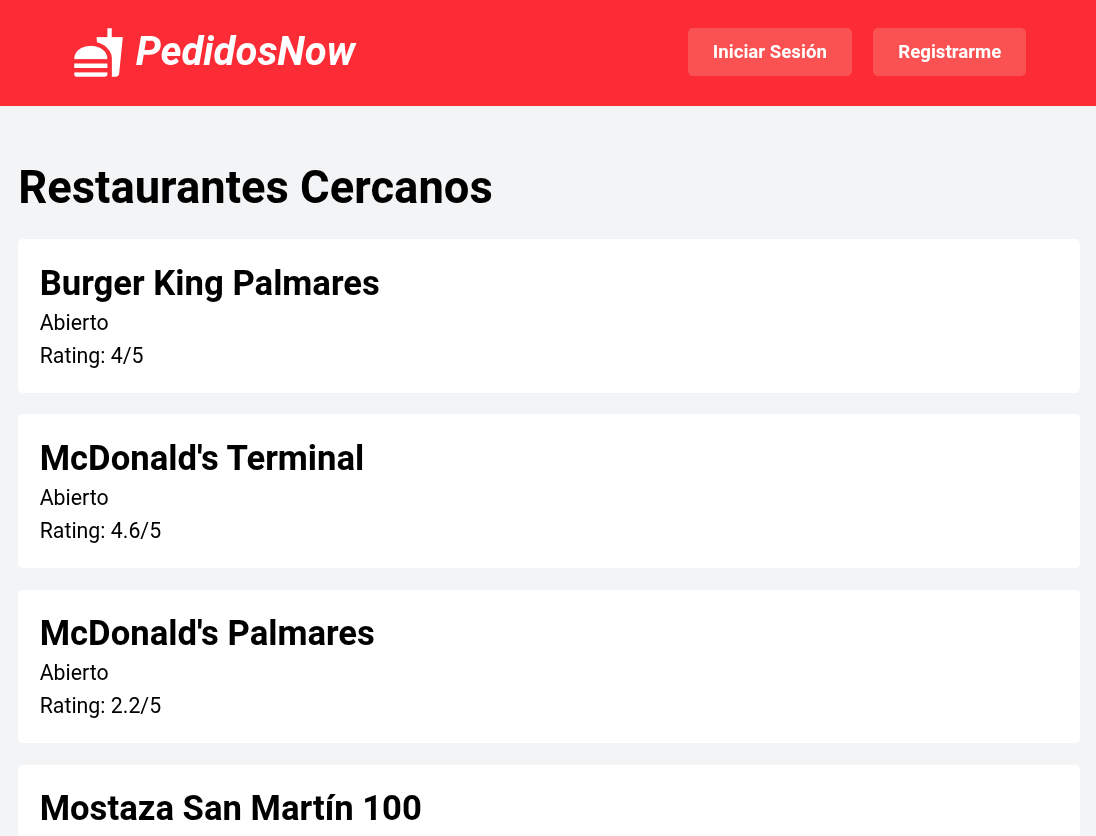
\includegraphics[width=10cm]{./img/public-locations.png}
    \caption{Pantalla de inicio.}
\end{figure}

Si hacemos click en una sucursal, podremos observar su menú, tal como lo muestra la siguiente figura. La pantalla indica el nombre de la sucursal, si está abierta o cerrada, su rating promedio, y los ítems de su menú. Para cada item se indica su nombre, categoría, descripción y precio. La funcionalidad del botón ``Comprar'' no está implementada.

\begin{figure}[H]
    \centering
    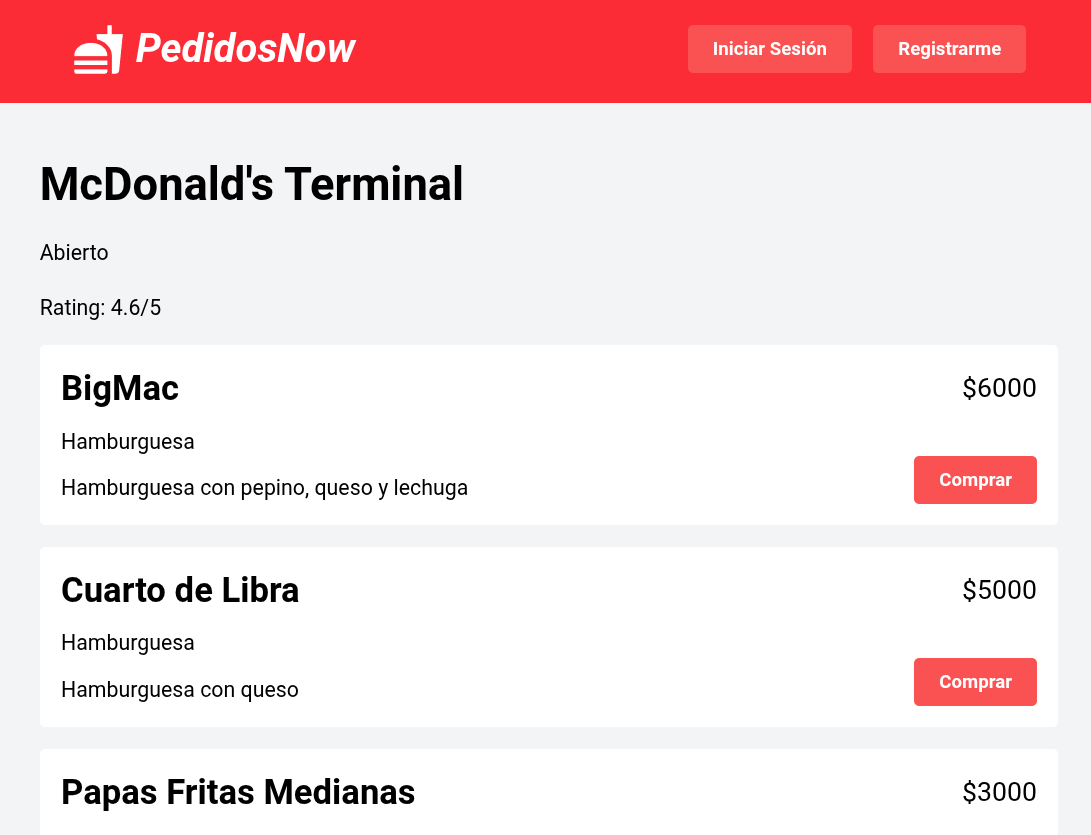
\includegraphics[width=10cm]{./img/public-items.png}
    \caption{Pantalla de menú de sucursal.}
\end{figure}

Para poder hacer modificaciones en los datos del sistema, debemos iniciar sesión o registrarnos. El sistema solo permitirá modificar aquellos recursos que sean del propio usuario, y no aquellos de otros usuarios. Para ello, hacemos click en el botón ``Iniciar Sesión'' o ``Registrarme'' en el encabezado de la página. Se abrirá una página como la de la siguiente figura.

\begin{figure}[H]
    \centering
    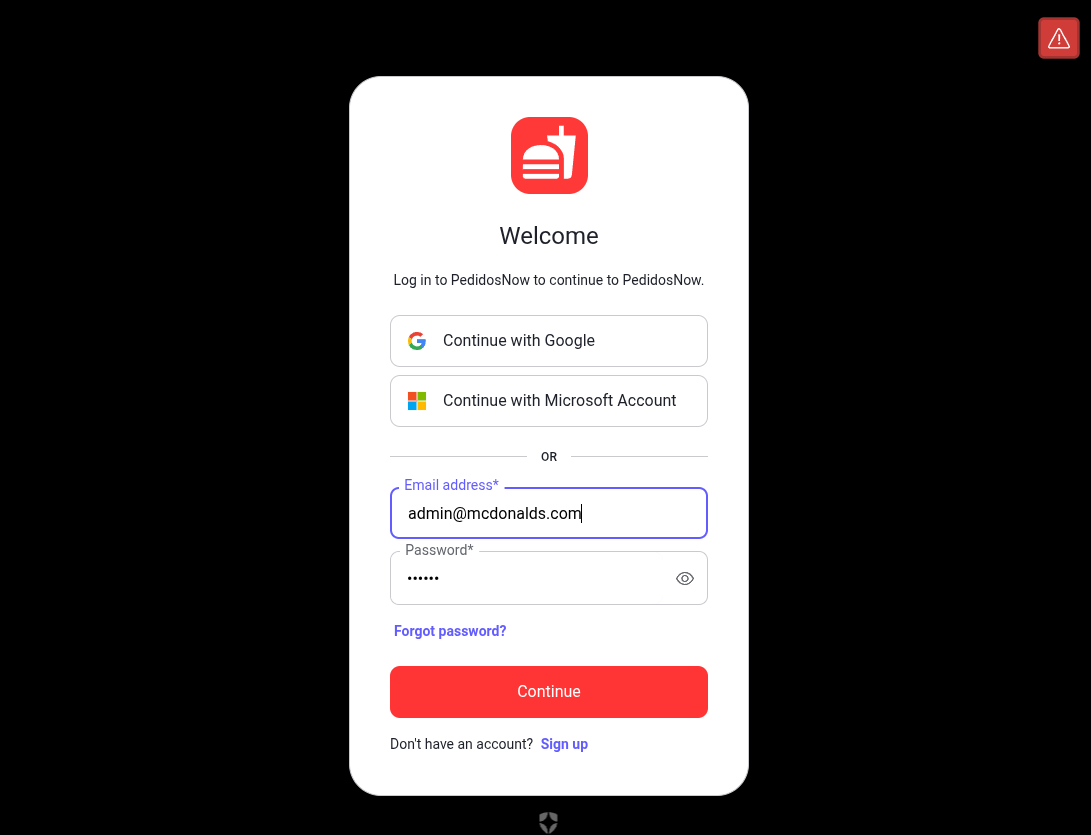
\includegraphics[width=10cm]{./img/login.png}
    \caption{Pantalla de inicio de sesión / registro.}
\end{figure}

En caso de crear un usuario nuevo, una vez autenticado, será redirigido a un formulario para completar su registro, como el de la siguiente figura, donde se deberá indicar el nombre de la cadena de restaurantes, y el domicilio legal.

\begin{figure}[H]
    \centering
    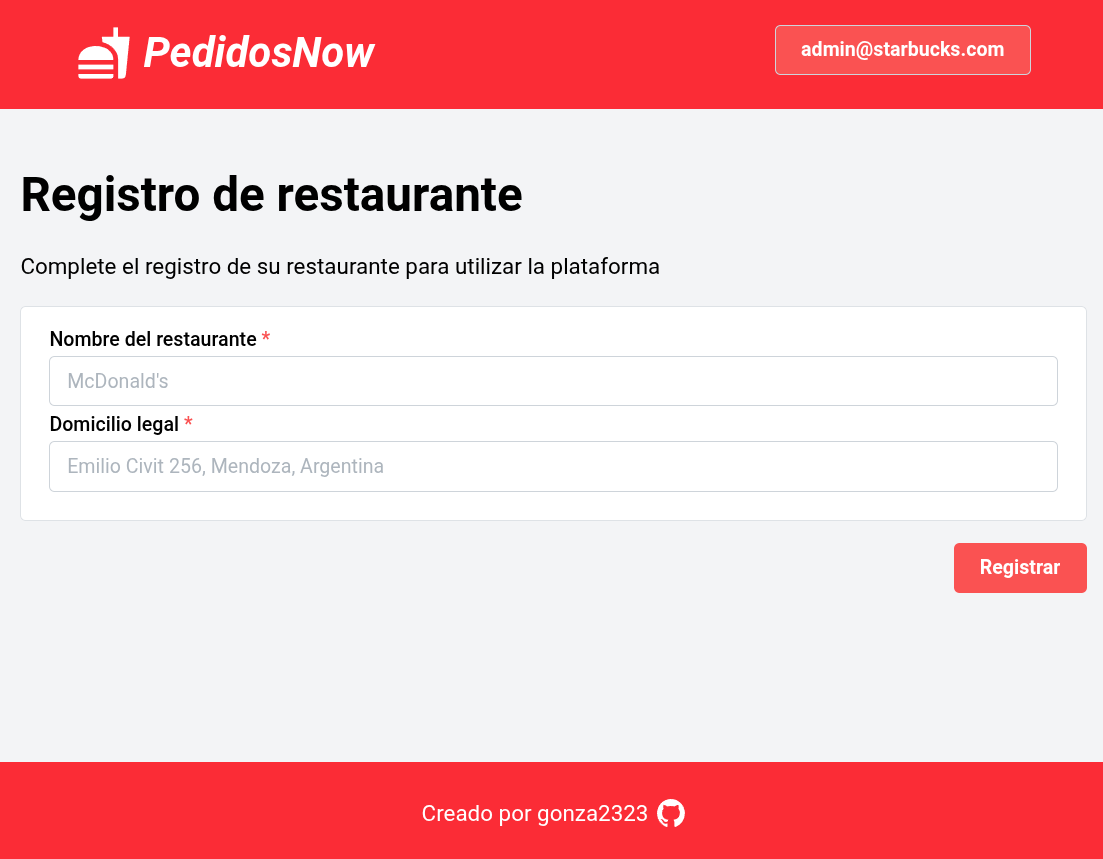
\includegraphics[width=10cm]{./img/login-form.png}
    \caption{Pantalla de registro de nuevo restaurante.}
\end{figure}

Una vez registrado y autenticado el usuario, se indicará el nombre del restaurante en el encabezado de la página, como se muestra en la siguiente figura. Si se hace click sobre el mismo, se abrirá un menú desplegable con opciones para ir a la página de administración de sucursales, y cerrar sesión.

\begin{figure}[H]
    \centering
    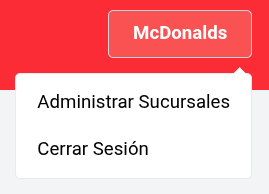
\includegraphics[width=4cm]{./img/dropdown.png}
    \caption{Menú desplegable para usuarios autenticados.}
\end{figure}

Si el usuario hace click en ``Administrar Sucursales'', será redirigido a una página como la de la siguiente figura. En la misma, se indican las sucursales de su restaurante, sus nombres, rating promedio, y si están abiertas o cerradas. Para cada una de ellas, hay botones para abrir, cerrar, editar o borrar esa sucursal en particular. También hay botones para añadir una nueva sucursal, o generar un reporte de los ingresos generados por cada una.

\begin{figure}[H]
    \centering
    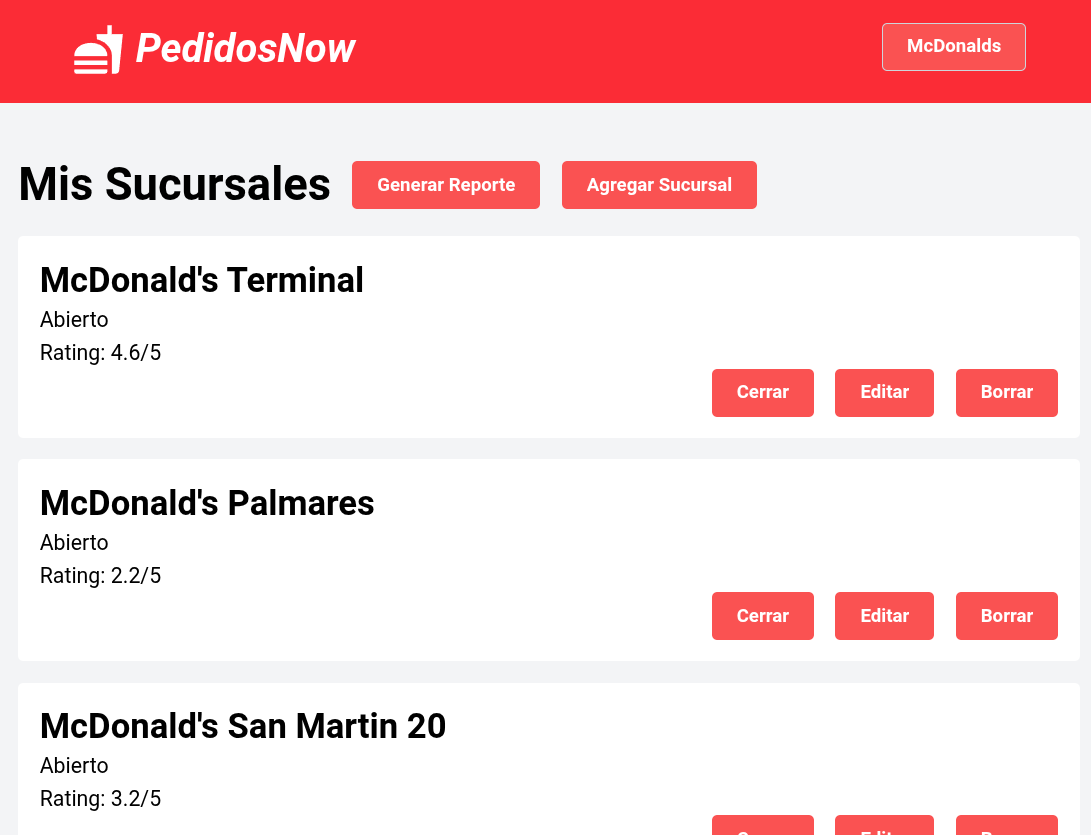
\includegraphics[width=10cm]{./img/locations.png}
    \caption{Página de gestión de sucursales.}
\end{figure}

Si el usuario hace click en ``Agregar Sucursal'', se abrirá un formulario como el de la siguiente figura. El usuario debe completar el nombre y los campos de dirección de la misma y presionar ``Agregar''.

\begin{figure}[H]
    \centering
    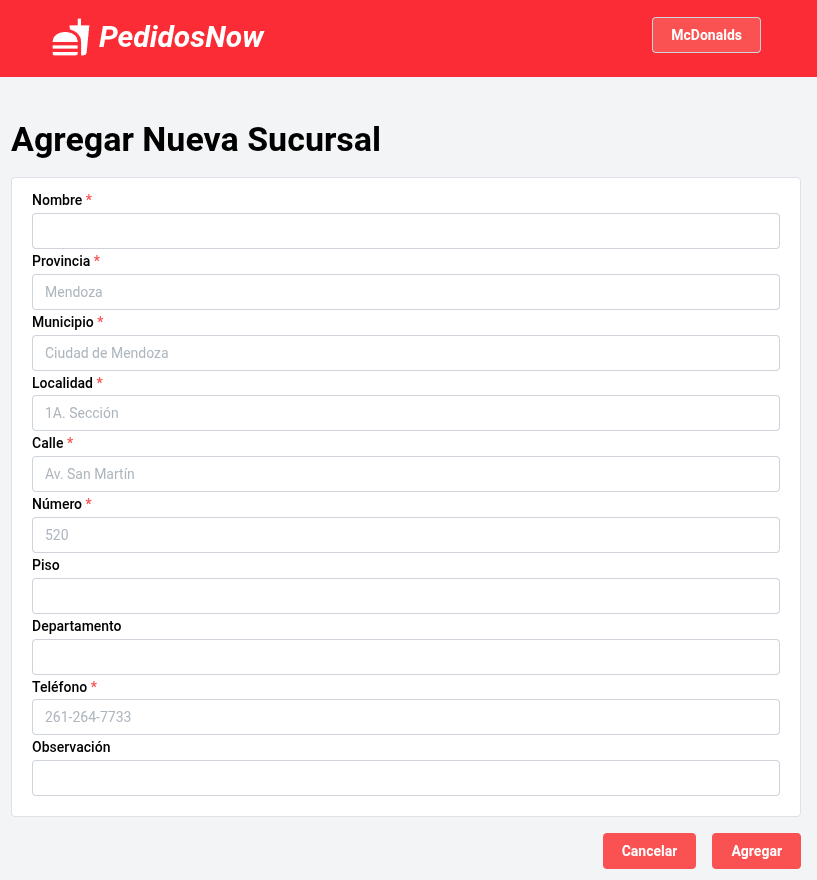
\includegraphics[width=10cm]{./img/locations-add.png}
    \caption{Formulario de alta de sucursal.}
\end{figure}

Si en la pantalla de gestión de sucursales, el usuario hace click en el botón ``Editar'' de alguna sucursal, será redirigido a un formulario para editar su nombre y dirección, como se muestra en la siguiente figura.

\begin{figure}[H]
    \centering
    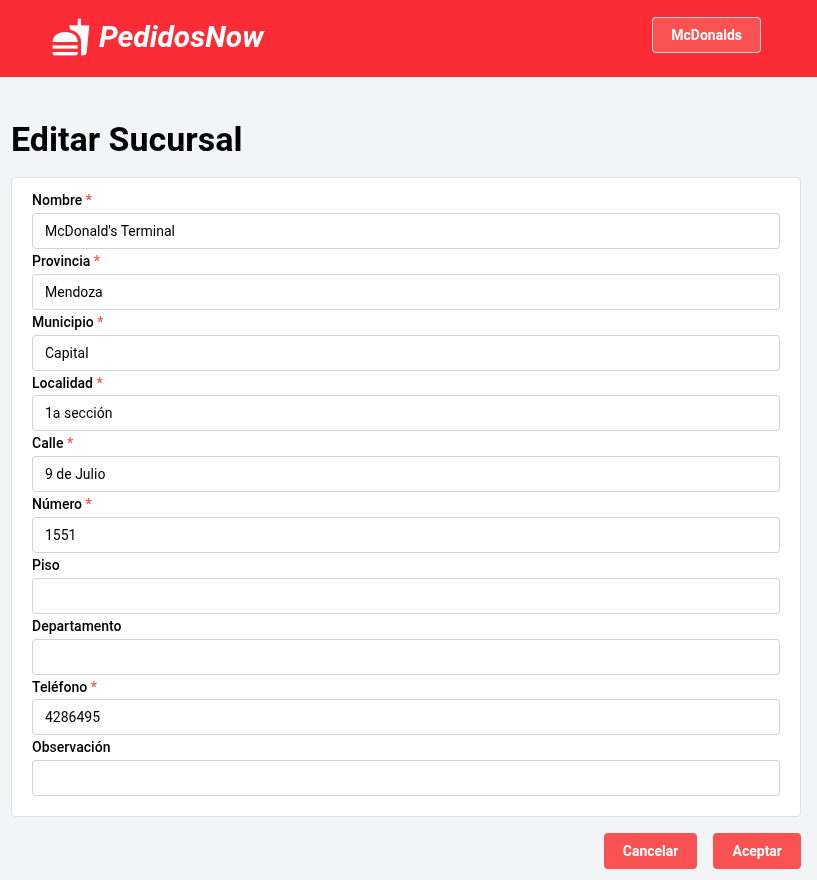
\includegraphics[width=10cm]{./img/location-edit.png}
    \caption{Formulario de modificación de sucursal.}
\end{figure}

Si en la pantalla de gestión de sucursales, el usuario hace click sobre alguna sucursal, será redirigido a la pantalla de gestión de menú de esa sucursal, donde podrá agregar, editar y modificar ítems del menú de la misma. Tal pantalla se muestra en la siguiente figura. En la misma se indican el nombre de la sucursal en cuestión, si está abierta o cerrada, su rating promedio, y los ítems de su menú. Para cada ítem, se indica su nombre, categoría, descripción, precio y disponibilidad. A su vez, cada ítem cuenta con botones para cambiar su disponibilidad, modificar sus datos y borrarlo. Al final de la página, encontramos un botón para agregar un nuevo ítem al menú.

\begin{figure}[H]
    \centering
    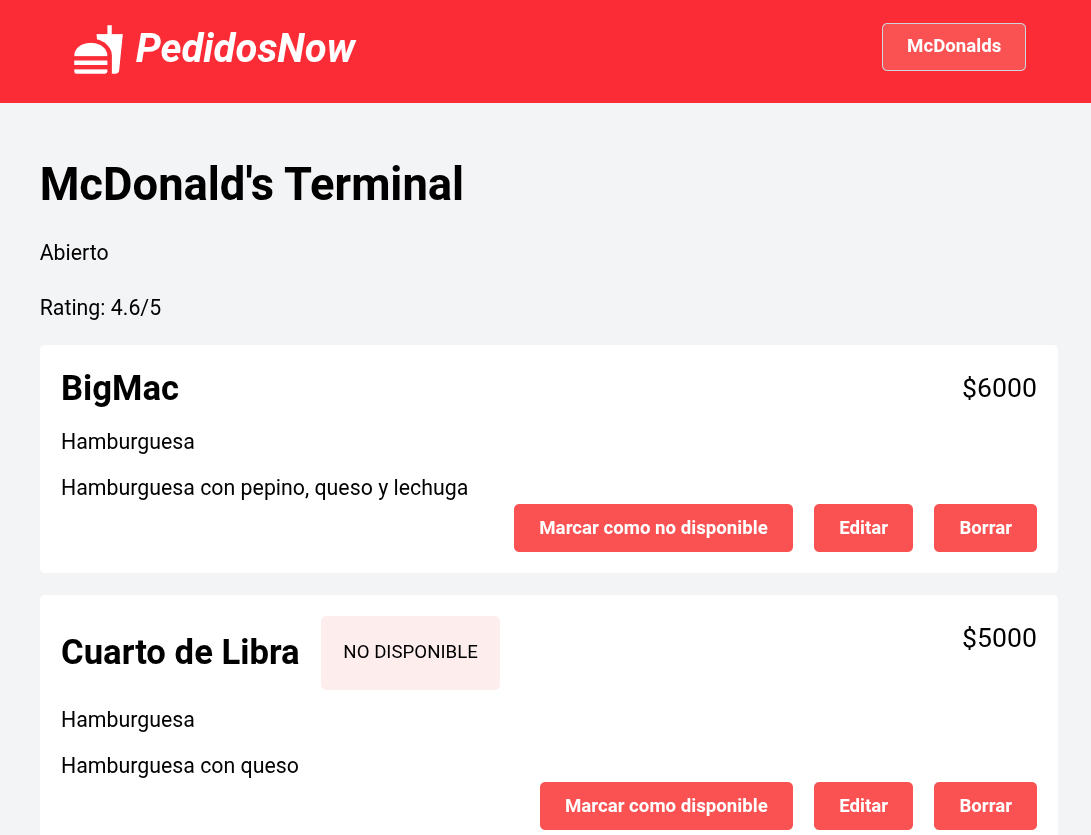
\includegraphics[width=10cm]{./img/items.png}
    \caption{Pantalla de gestión de menú de sucursal.}
\end{figure}

Si hacemos click en ``Agregar ítem al menú'', se abrirá un formulario como el de la siguiente figura. En el mismo, el usuario debe indicar el nombre, descripción, precio y categoría (de las cargadas ya en la base de datos), del ítem a agregar. Una vez listo, debe presionar ``Confirmar''.

\begin{figure}[H]
    \centering
    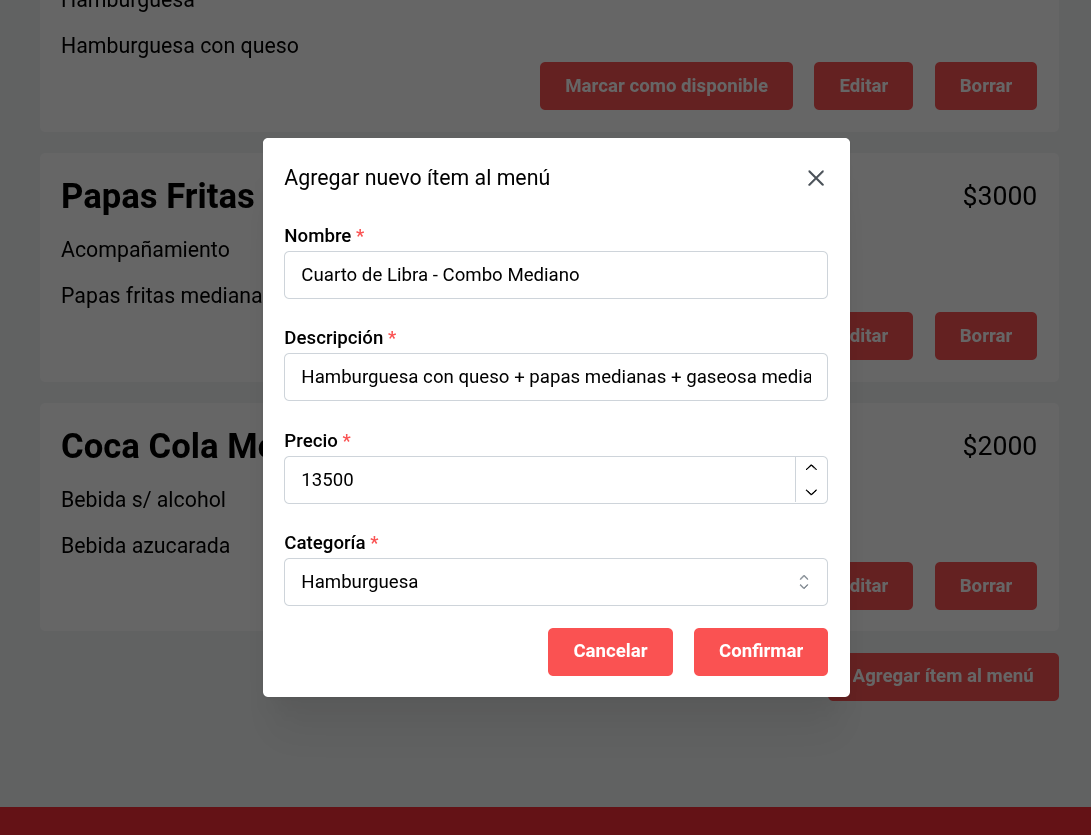
\includegraphics[width=10cm]{./img/item-add.png}
    \caption{Formulario de alta de ítem de menú.}
\end{figure}

Si hacemos click en el botón ``Editar'' de algún ítem del menú, se abrirá un formulario similar al anterior para modificar los datos del ítem en cuestión, tal como se muestra en la siguiente figura.

\begin{figure}[H]
    \centering
    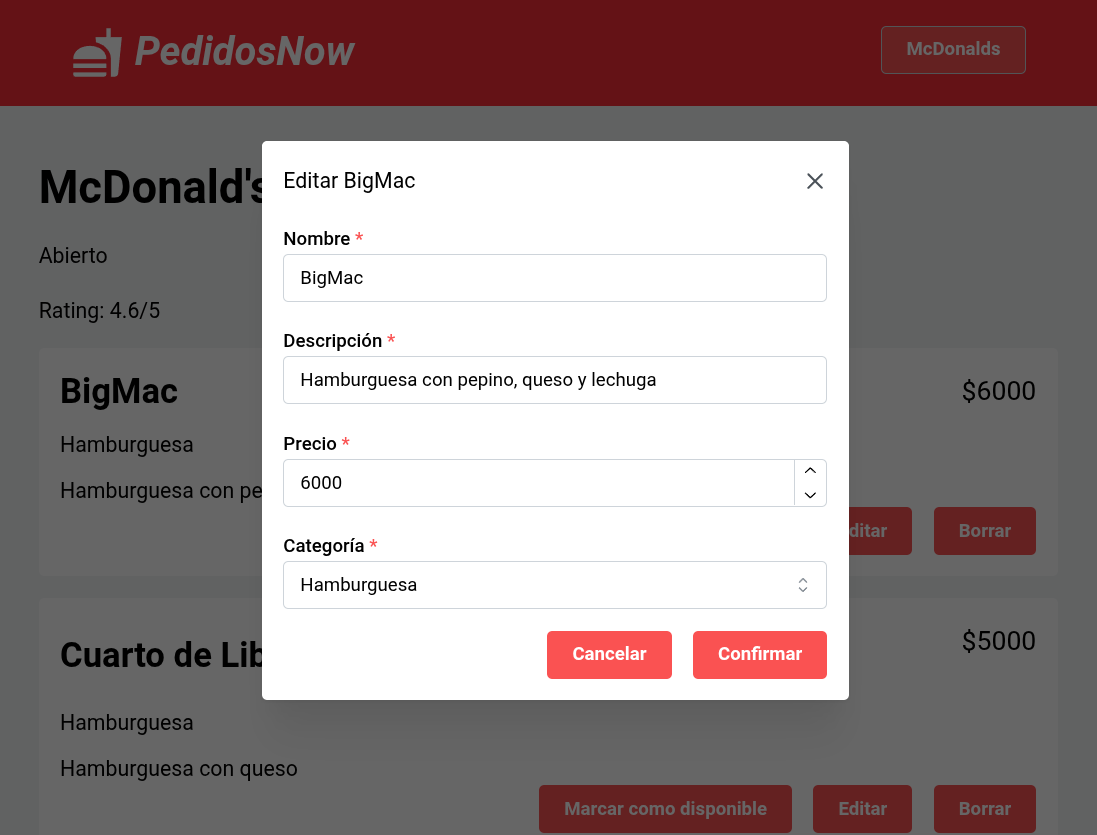
\includegraphics[width=10cm]{./img/item-edit.png}
    \caption{Formulario de modificación de ítem de menú.}
\end{figure}

Por otro lado, si en la pantalla de gestión de sucursales, hacemos click en el botón ``Generar Reporte'', se generará un reporte en formato PDF como el de la siguiente figura. El mismo contiene el nombre de la cadena de restaurantes, la dirección de mail asociada, y una tabla de las sucursales cargadas. Para cada sucursal, se indica si está actualmente abierta o cerrada, su rating promedio (si es que hay suficientes reseñas), la cantidad de pedidos que ha entregado, el monto promedio de los mismos, y la cantidad de ingresos totales que ha generado durante su existencia.

\begin{figure}[H]
    \centering
    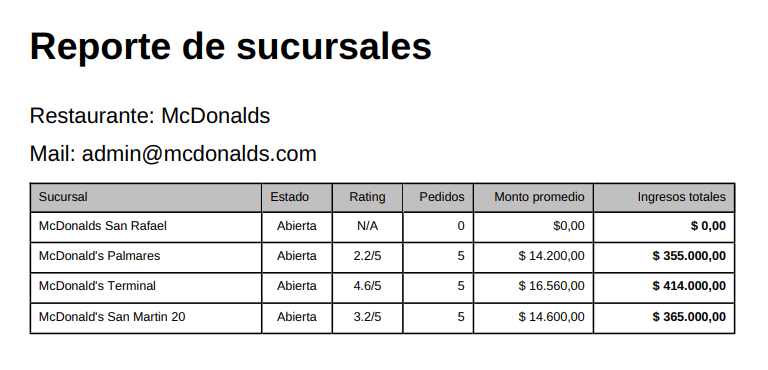
\includegraphics[width=10cm]{./img/report.png}
    \caption{Reporte de ingresos por sucursal.}
\end{figure}

Si en lugar de iniciar sesión como un restaurante, iniciamos sesión con una cuenta de administrador, el menú desplegable indicará ``Admin'', y ofrecerá la opción de ``Administrar Backups'', tal como se indica en la siguiente figura.

\begin{figure}[H]
    \centering
    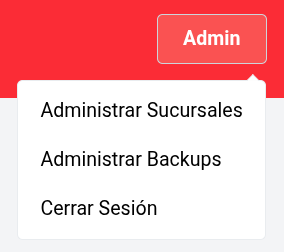
\includegraphics[width=4cm]{./img/admin-dropdown.png}
    \caption{Menú desplegable para administrador.}
\end{figure}

Si hacemos click en tal opción, se abrirá una pantalla como la de la siguiente figura. En la misma podemos ver una lista de los backups ya creados. Para cada uno, se indica su nombre, el cual incluye la hora y fecha de creación, y botones para descargar, eliminar o restaurar esa copia de seguridad. También hay botones para crear un nuevo backup y para subir un archivo de copia de seguridad.

\begin{figure}[H]
    \centering
    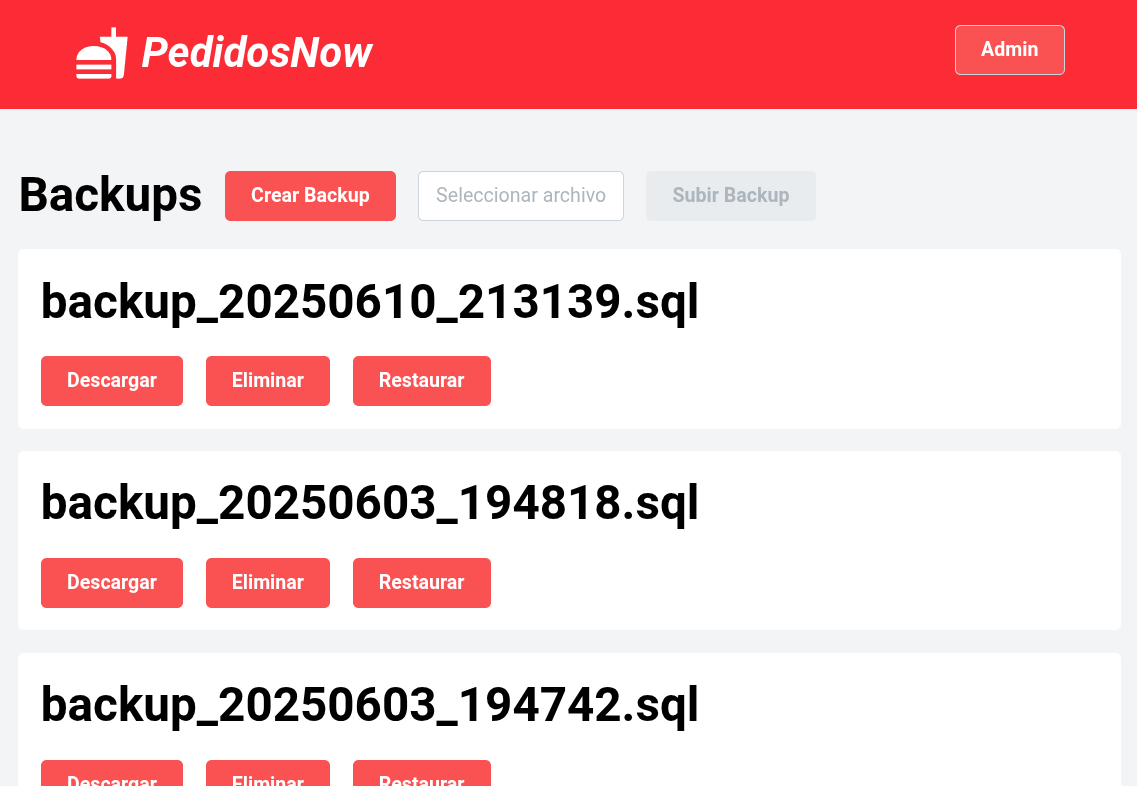
\includegraphics[width=10cm]{./img/admin-backups.png}
    \caption{Pantalla de gestión de copias de seguridad.}
\end{figure}